\documentclass[border=10pt]{standalone}
\usepackage{tikz}
\usepackage{circuitikz}
\usetikzlibrary{positioning, backgrounds, calc}

\begin{document}

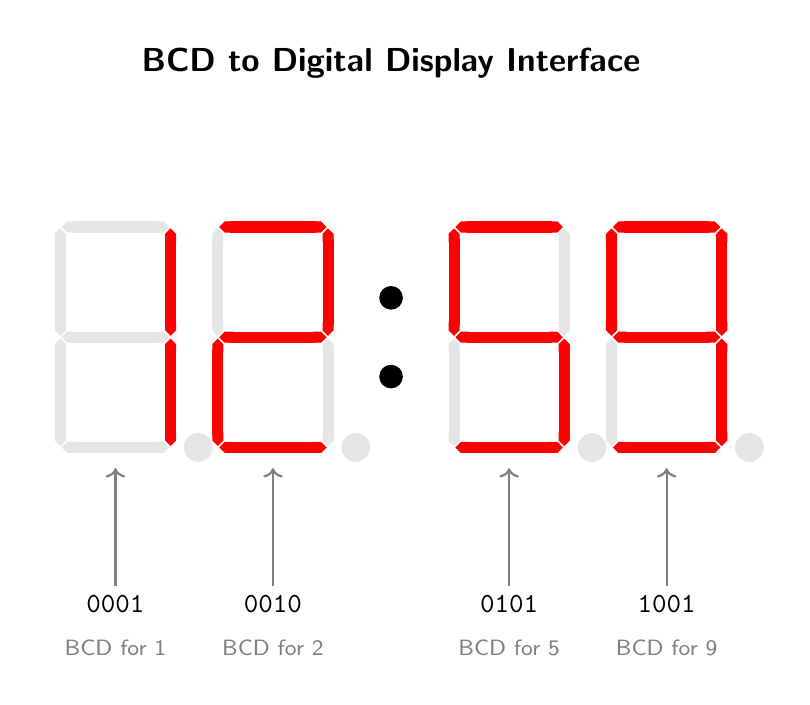
\begin{tikzpicture}[
    background rectangle/.style={fill=white},
    show background rectangle,
    digit/.style={draw, thick, rectangle, minimum width=1.5cm, minimum height=2.5cm, rounded corners},
    bcd/.style={font=\ttfamily\small, align=center},
    label/.style={font=\sffamily\footnotesize, gray}
]

    % Digits for 12:59
    % H1 (1)
    \node[seven segment val=1 dot off box off, scale=2.5] (d1) at (-3, 0) {};
    % H2 (2)
    \node[seven segment val=2 dot off box off, scale=2.5] (d2) at (-1, 0) {};
    
    % Colon
    \fill[black] (0.5, 0.5) circle (0.15);
    \fill[black] (0.5, -0.5) circle (0.15);
    
    % M1 (5)
    \node[seven segment val=5 dot off box off, scale=2.5] (d3) at (2, 0) {};
    % M2 (9)
    \node[seven segment val=9 dot off box off, scale=2.5] (d4) at (4, 0) {};

    % BCD Values below
    % 1 -> 0001
    \node[below=1.5cm of d1] (b1) {\texttt{0001}};
    \node[label, below=0.1cm of b1] {BCD for 1};
    \draw[->, thick, gray] (b1.north) -- (d1.south);

    % 2 -> 0010
    \node[below=1.5cm of d2] (b2) {\texttt{0010}};
    \node[label, below=0.1cm of b2] {BCD for 2};
    \draw[->, thick, gray] (b2.north) -- (d2.south);

    % 5 -> 0101
    \node[below=1.5cm of d3] (b3) {\texttt{0101}};
    \node[label, below=0.1cm of b3] {BCD for 5};
    \draw[->, thick, gray] (b3.north) -- (d3.south);

    % 9 -> 1001
    \node[below=1.5cm of d4] (b4) {\texttt{1001}};
    \node[label, below=0.1cm of b4] {BCD for 9};
    \draw[->, thick, gray] (b4.north) -- (d4.south);

    % General Title
    \node[above=1.5cm of d2, xshift=1.5cm, font=\bfseries\sffamily\large] {BCD to Digital Display Interface};

\end{tikzpicture}

\end{document}
